\documentclass[11pt]{article}
\usepackage{amsmath,amssymb,color,float}
\usepackage{stmaryrd}
\usepackage{graphicx,psfrag,epsf}
\usepackage[authoryear]{natbib}
\usepackage{fullpage,setspace}
\usepackage{subcaption}
\usepackage{changepage}
\usepackage{listings}

\setlength{\oddsidemargin}{.15in} 
\setlength{\textwidth}{6.25in}
\setlength{\topmargin}{-0.25in}
\setlength{\headheight}{-0.15in}
\setlength{\textheight}{8.9in} 

\usepackage{amssymb}
\linespread{1.25}
\title{NPMLE for Binary Response Models with Random Coefficients}
\author{Kevin Collins and Michael Lightfoot}
\date{December 2023}

\begin{document}

\maketitle
\section{Introduction}

\indent

The objective of \textit{Nonparametric Maximum Likelihood Methods for Binary Response Models With Random Coefficients}, \cite{NPMLE} is to introduce a computationally tractable method for employing NPMLE in single-index binary response models with random coefficients. Gu and Koenker first develop a nonparametric MLE approach to the problem and then utilize tools from computational geometry to improve the feasibility of recovering these estimators for binary response models. They then analyze the theoretical properties of the NMLPEs dveloped. We find the topics of computational geometry and the theoretical framework of NPMLEs to be interesting in their own right, and further believe this intersection of computation and theory to be central to modern statistical inference.

The premise is quite simple. Previously we have discussed censored data with thresholds, where a censored value is given if below (or above) a given threshold. In the case of a binary response, we only see a value $y_i$ which equals either 0 or 1. Now what makes this problem in this paper unique is the structure of the underlying process that generates $y_i$.
\[
y_i = 1\{x_i'\beta_i + w_i'\theta \geq 0\}
\]

We observe $y_i$ and covariates $(x_i,w_i)$. The obvious task is to make inferences about the coefficients $\theta$ and $\beta_i$. However, this model complicates itself by having $\theta$ be a fixed, vector-valued parameter, while $\beta_i$ is random.

Let $\beta_i \sim F_0 \text{ iid}$. Then, our inferential task of interest becomes estimating the set $(\theta_0,F_0)$. \cite{NPMLE} propose a nonparametric approach to this problem. For illustrative purposes, let us consider the univariate case for a moment.

\subsection{Univariate Example}

\indent

To simplify the problem, assume we observe some $y_i$ that comes from the generating mechanism
\[
y_i=1\{\beta_i\geq w_i\}
\]
where $\beta_i\perp w_i$. Now, we approach this problem by visualizing our data on the real line. We let each $y_i$ partition the real line into two sections by imposing an interval 
\[
R_i=(-\infty,w_i] \text{ if } y_i=1 
\]
\[
R_i=[w_i,\infty) \text{ if } y_i=0
\]
Thus, we can see how each observed data point partitions the real line into $R_i$ and $R_i^c$.

Now, after constructing partitions from each $(y_i,w_i)$, we have a collection intervals defined by the $w_i$ and an allotment of "mass" in one direction or the other. From this, we can begin to see we can construct a PMF-esque structure. Now, let $u_{(i)}$ be the $i^{th}$ order statistic from $w_1,\dots,w_n$. For a given interval $[u_{(i)},u_{(i+1)})$, we sum up
\[
C_i=\sum_j y_j1\{w_j\geq u_{(i+1)}\} + (1-y_j)1\{w_j\leq u_{(i+1)}\} 
\]
In order to construct a likelihood we look at this collection of intervals and weights and see it begins to resemble a categorical distribution. Thus, returning to our goal of inferring the distribution of $\beta_i$, we turn to the following optimization problem
\[
\text{arg}\max_{p_1,\dots,p_{n+1}} \sum_{j=1}^{n+1} C_jp_j
\]
This histogram shape and the probabilities that result from the above optimization provide an estimate for the distribution of $\beta_i$.

\subsection{Multivariate Extension}

\indent

The univariate example comes with the wonderful property that we can easily visualize the partitioning and intervals our data creates on the real line. This carries over somewhat into the second-dimension, but as soon as we go into higher dimensions the geometry becomes more complicated, dealing with hyperplanes rather than intervals. 

However, the complicated geometry does not throw out the powerful intuition we gain from the univariate case. Turning back to our original model, each observed instance $(y_i,x_i,w_i)$ divides the higher dimensional space into two half-spaces, the exact same way that each $y_i$ created $R_i$ and $R_i^c$ in our univariate setting!

Instead of $R_i$, we define a new space
\[
H(x_i,w_i,\theta)=\{\beta:x_i'\beta+w_i'\theta\geq0\}
\]
And so, in a similar manner of mass attribution as in the univariate case, this leads to the nonparametric MLE:

\[
(\hat F_n,\hat\theta_n)=\text{arg}\max_{\Theta\times\mathcal{F}} \frac{1}{n}\sum_{i=1}^ny_i\log\{\mathbb P_F(H(x_i,w_i,\theta))\}
\]
\[
+(1-y_i)\log\{1-\mathbb P_F(H(x_i,w_i,\theta))\}
\]

It may not come as a surprise, but this is not a trivial optimization problem. However, the authors also provide a computationally tractable approach utilizing some tools from combinatorial geometry. For the rest of this blog, we will state and flesh out the proofs of the identifiability and strong consistency of the NPMLE in Section 2, and then provide results from a simulation study in Section 3.


\section{Identifiability and Strong Consistency of the Proposed Estimator}

\indent

We now introduce two more bits of notation to make expressions more concise. First, we say $\gamma=(F,\theta)$, i.e. our parameters of interest. Secondly, let

\[
p(y,x,w,\gamma)=y\mathbb{P}_F(H(w,x,\theta))+(1-y)(1-\mathbb{P}_F(H(w,x,\theta)))
\]

Note that this expression is essentially the likelihood function from earlier presented in a slightly different manner.

Similar to when we proved the strong consistency of the MLE in class, we make three assumptions.
\begin{enumerate}
    \item The random vectors $(Z,V,W)$ and $\beta_i$ are independent.
    \item The parameter space $\Theta$ is a compact subset of a Euclidean space and $\theta_0\in\Theta$. Let the set $\mathcal F$ be the space of probability distributions for $\beta_i$ supported on a compact set in $\mathbb{R}^d$.
    \item The random variable $V$ conditional on $(W,Z)$ is absolutely continuous and has full support on $\mathbb{R}$ and the random variables $Z$ conditional on $W$ are absolutely continuous and has full support on $\mathbb{R^d}$.
\end{enumerate}

From these, we can make the following two statements.

\paragraph{Theorem 1} Under Assumptions 1-3, $(\theta_0,F_0)$ is identified.

\paragraph{Theorem 2} If $\{(y_i,x_i,w_i):i=1,2,\dots,n\}$ is an iid sample from $p(y,x,w,\theta_0,F_0)$, under assumptions 1-3, then $(\hat \theta_n,\hat F_n)$ is strongly consistent.

\subsection{Proof of Theorem 1}

\indent

In order to prove identifiability, we wish to show that both $\theta_0$ and $F_0$ can be identified. A small note is that estimability of this method requires some restrictions on $\beta$, so we rewrite our model as
\[
y_i1\{w_i'\theta_0 + \beta_{1i} + z_i'\beta_{-1i}\}
\]
First, let $U=W'\theta_0 + \beta_{1i} + Z'\beta_{-1i}$ be a random variable. Under Assumptions 1 and 3, we can identify the distribution of $U|(W,Z)$  over all of its support. Then, if we fix $Z=z$ and consider two instances $w_1\neq w_2$, we can easily identify $\theta_0$.

Now in order to show that the distribution $F_0$ of $\beta_i$ is identifiable, we take an approach of looking at the characteristic function of $U|(W,Z)$. This is defined as
\[
\phi_{U|(W,Z)}(t|w,z)=\mathbb E[e^{itU}|(W,Z)]
\]
\[
=\mathbb E[e^{it(w'\theta_0+\beta_{1i}+z'\beta_{-1i}}|(W,Z)]
\]
Then, by the independence from Assumption 1,
\[
=e^{itw'\theta_0}\mathbb E[e^{it(\beta_{1i}+z'\beta_{-1i}}|(W,Z)]
\]
\[
=e^{itw'\theta_0}\phi_\beta(t(1,z))
\]
Now we have an expression that isolates the characteristic function of $\beta$, so by observing variations of $z$, we are able to identify $\beta$. This concludes the proof, which the authors note is similar to the argument for the Cramér-Wold device.

\subsection{Proof of Theorem 2}

\indent

In order to prove Theorem 2, we first need to state and prove two lemmas that will come in handy.

\subsubsection{Lemma 1}

\paragraph{Claim} Under Assumptions 1-3, for any given $\gamma = (\theta,F)\in\Theta\times\mathcal{F}_0,$ let $\gamma_n=(\theta_n,F_n)$ be any sequence such that $\gamma_n \rightarrow \gamma$, then
\[
\lim_{\gamma_n\rightarrow\gamma}\mathbb{P}_{F_n}(H(x,w,\theta_n))=\mathbb{P}_F(H(x,w,\theta)) \text{  a.s.}
\]

\paragraph{Proof} We assumed that $\mathcal F_0$ is the set of all continous distributions on the support of $\beta$; thus, $\mathbb P_F$ is continuous for $F\in \mathcal F_0$. Additionally, we know that $w_i'\theta$ is continuous in $\theta$. Now consider $\epsilon >0$ and some sequence $\theta_n\rightarrow\theta$. Then, as we are just composing two continuous functions, there exists $N_1$ such that for all $n\geq N_1$ and a given $F$,
\[
|\mathbb P_{F}(H(x,w,\theta_n))-\mathbb P_F(H(x,w,\theta_0))|<\epsilon
\]
Now we wish to show a similar result, but for a sequence $F_n\rightarrow F$. The authors employ a measure theoretic result, called the Portmanteau Theorem, which gives us that
\[
F_n\rightarrow F \implies \mathbb P_{F_n}(H(x,w,\theta))\rightarrow \mathbb P_{F}(H(x,w,\theta))
\]
We will not give details on this theorem, but just note that it essentially gives various equivalent statements surrounding the idea of convergence in distribution. 

Finally, let $\epsilon>0$ be given and choose $N_1$ and $N_2$, s.t. for $n_1\geq N_1$, $|\mathbb P_{F}(H(x,w,\theta_n))-\mathbb P_F(H(x,w,\theta_0))|<\epsilon/2$ and for $n_2\geq N_2$, $|\mathbb P_{F_n}(H(x,w,\theta))-\mathbb P_F(H(x,w,\theta))|<\epsilon/2$. WLOG, we say that $N_2\geq N_1$. Then, it is clear to see that for all $n\geq N_2$
\[
|\mathbb P_{F_n}(H(x,w,\theta_n)) - \mathbb P_{F}(H(x,w,\theta))|
\]
\[
=|\mathbb P_{F_n}(H(x,w,\theta_n)) - \mathbb P_{F_n}(H(x,w,\theta)) + \mathbb P_{F_n}(H(x,w,\theta)) - \mathbb P_{F}(H(x,w,\theta))|
\]
\[
\leq |\mathbb P_{F_n}(H(x,w,\theta_n)) - \mathbb P_{F_n}(H(x,w,\theta))| + |\mathbb P_{F_n}(H(x,w,\theta)) - \mathbb P_{F}(H(x,w,\theta))|
\]
\[
<\epsilon/2+\epsilon/2=\epsilon
\]
Therefore, because $\epsilon$ is arbitrary, we have shown Lemma 1.

\subsubsection{Lemma 2}

\paragraph{Claim} Under Assumptions 1-3, for any $\gamma\neq\gamma^*$ with $\gamma^*=(F_0,\theta_0)$, the truth, there exists $\epsilon>0$ such that
\[
\mathbb{E}^*\{[\log\{p(y,x,w,\Gamma_\epsilon (\gamma))/p(y,x,w,\gamma^*)\}]^+\}<\infty
\]
where $\mathbb{E}^*$ denotes the expectation taken with respect to $p(y,x,w,\gamma^*)$ and
\[
p(y,x,w,\Gamma_\epsilon (\gamma)) = \sup_{\tilde\gamma\in\Gamma_\epsilon(\gamma)} p(y,x,w,\tilde\gamma)
\]
where $\Gamma_\epsilon(\gamma)$ is an open ball around $\gamma$ with radius $\epsilon$.

\paragraph{Proof} As it is a probability function, we know that $0\leq\mathbb P_F(H(x,w,\theta))\leq1$, and therefore,
\[
p(1,x,w,\Gamma_\epsilon (\gamma))/p(1,x,w,\gamma^*) = \mathbb P_{F_\gamma}(H(x,w,\theta))/\mathbb P_{F_0}(H(x,w,\theta))
\]
\[
\leq 1/\mathbb P_{F_0}(H(x,w,\theta))
\]
Similarly,
\[
p(0,x,w,\Gamma_\epsilon (\gamma))/p(0,x,w,\gamma^*) \leq 1/(1-\mathbb P_{F_0}(H(x,w,\theta)))
\]
Thus, we can see that
\[
\mathbb{E}^*\{[\log\{p(y,x,w,\Gamma_\epsilon (\gamma))/p(y,x,w,\gamma^*)\}]^+\}
\]
\[
\leq\int\bigg[-\mathbb P_{F_0}(H(z,w,\theta))\log\mathbb P_{F_0}(H(z,w,\theta))
\]
\[
-(1-P_{F_0}(H(z,w,\theta)))\log\mathbb (1-P_{F_0}(H(z,w,\theta)))\bigg]dG(z) <\infty
\]
where $G(z)$ is the joint distribution of $(x,w)$. This proves Lemma 2.

\subsubsection{Proof of Theorem 2 Cont.}

\indent

Now that we have proved Lemmas 1 and 2, we will bring them into the fold to prove the strong consistency of the NPMLE. The remainder of the proof has some technical details that use more Measure Theoretic results and are beyond the scope of this course, so instead we focus on a high-level roadmap of the proof. 

First, Lemma 1 gives us that 
\[
\lim_{\epsilon\rightarrow0}p(y,x,w,\Gamma_{\epsilon}(\gamma))= p(y,x,w,\gamma)
\]
We now note that $\log\{p(y,x,w,\Gamma_\epsilon (\gamma))/p(y,x,w,\gamma^*)\}$ is a monotone increasing function on a compact space. This, in combination with Lemma 1, and two other convergence results (dominated convergence and Fatou's Lemma) gives us that the following limit exists with given bound
\[
\lim_{\epsilon\rightarrow0}\mathbb{E}^*\{\log\{p(y,x,w,\Gamma_\epsilon (\gamma))/p(y,x,w,\gamma^*)\}\}
\]
\[
\leq \mathbb{E}^*\{\log\{p(y,x,w,\gamma)/p(y,x,w,\gamma^*)\}\} < 0
\]
Ultimately, what this implies is that $\gamma^*$, the true value, uniquely maximizes the nonparametric log-likelihood function. They complete the proof of almost sure convergence by considering a finite subcover of the complementary set $\Gamma_{\epsilon}(\gamma^*)^c$: $\Gamma_1,\dots,\Gamma_j$, i.e. we can describe the set outside the neighborhood of $\gamma^*$ with this finite collection. Now, we return to our likelihood function and consider all possible $\gamma$ values
\[
\sup_{\gamma\in\Gamma_\epsilon(\gamma^*)} \frac{1}{n}\sum_{i=1}^n\log\{p(y,x,w,\gamma)/p(y,x,w,\gamma^*)\}
\]
\[
\leq \max_j\frac{1}{n}\sum_{i=1}^n\log\{p(y,x,w,\Gamma_j)/p(y,x,w,\gamma^*)\}
\]
Now, from Lemma 2, we know that the first moment exists, so we can apply the Strong Law of Large Numbers to get that
\[
\max_j\frac{1}{n}\sum_{i=1}^n\log\{p(y,x,w,\Gamma_j)/p(y,x,w,\gamma^*)\}
\]
\[
\rightarrow^{wp1} \max_j \mathbb{E}^*\{\log\{p(y,x,w,\Gamma_j)/p(y,x,w,\gamma^*)\}\} <0
\]
This essentially means that maximizing with under the ground truth $\gamma^*$ will necessarily drive our estimator to converge almost surely to the truth. Therefore, we have shown that
\[
(\hat \theta_n, \hat F_n) \rightarrow (\theta_0,F_0) \text{ a.s.}
\]


\section{Simulation Study}

\indent

In this section, we would like to examine the performance of the various methods evaluated in this paper under different settings in order to see if the reported results change. Additionally, we want to examine the computational efficiency of the methods considered in greater detail. It is also worth noting that the simulation results in the paper report four digits of their measurements with respect to Monte Carlo simulations of only 100 simulations. The reported values for the following simulations will be rounded further than in the paper. 

The two main methods that Gu and Koenker compare their methods to are logistic regression and the method proposed by \cite{gautier2013nonparametric}. Central to this latter method is a deconvolution procedure via elegant Fourier–Laplace inversion formulas. A main critique of this method is the extensive number of tuning parameters, which the NPMLE does not require. One such parameter is the sieve dimension, which adjusts for overfitting. A high sieve dimension typically overfits the contours of the underlying distribution. These methods are all compared via the MAE and RMSE of predicted probabilities. Due to time constraints, 50 Monte Carlo simulations  with sample size $n = 100$ will be performed for all analyses. The time reported is the total computational time needed throughout the 50 Monte Carlo simulations to fit a given model.

\subsection{Point Masses}

\indent

The main simulation results presented in this paper are Monte Carlo simulations under a few different settings that were adapted from \cite{gautier2013nonparametric}. These simulations all have the goal of fitting the true underlying distribution. The first experiment considers the setting where the true underlying distribution is made up of two point masses. The setting in the paper examines equal point masses, so let's consider the case of point masses of unequal weights 0.9 and 0.1 as a more extreme example. These masses were still placed in the same points (0.7,-0.7,1) and (-0.7,0.7,1). The results for this first setting are reported in Table 1.   

\begin{table}[!htbp]
\begin{center}
\begin{tabular}{lrrrr}
\hline\hline
\multicolumn{1}{l}{}&\multicolumn{1}{c}{GK}&\multicolumn{1}{c}{NPMLE}&\multicolumn{1}{c}{NPMLEs}&\multicolumn{1}{c}{Logit}\tabularnewline
\hline
MAE&$0.17$&$  0.06$&$  0.12$&$0.22$\tabularnewline
RMSE&$0.23$&$  0.13$&$  0.18$&$0.35$\tabularnewline
Time&$8.84$&$205.06$&$205.06$&$0.04$\tabularnewline
\hline
\end{tabular}
\caption{Bivariate Point Mass Simulation Setting:  
Mean Absolute and Root Mean Squared Errors of Predicted Probabilities. 
The computational fitting times reported for NPMLE and NPMLEs are the same as
the smoothing occurs only during the prediction process.}
\label{tab.sim0a}
\end{center}
\end{table}

We see even when the point masses are not of equal size, the NPMLE method outperforms the method proposed by Gautier and Kitamura at this sample size. This is relatively expected as this setting is more suited to the NPMLE framework.  We also see that the proposed method takes much longer in computational time than both the GK method and logistic regression. Here the GK method used is the default as proposed in their paper. This discrepancy in computational time only grows with sample size. Contour plots of the corresponding density estimates for the GK and NPMLE methods can be seen in Figure 1 and Figure 2 respectively. 

\begin{figure}[H]
\centering
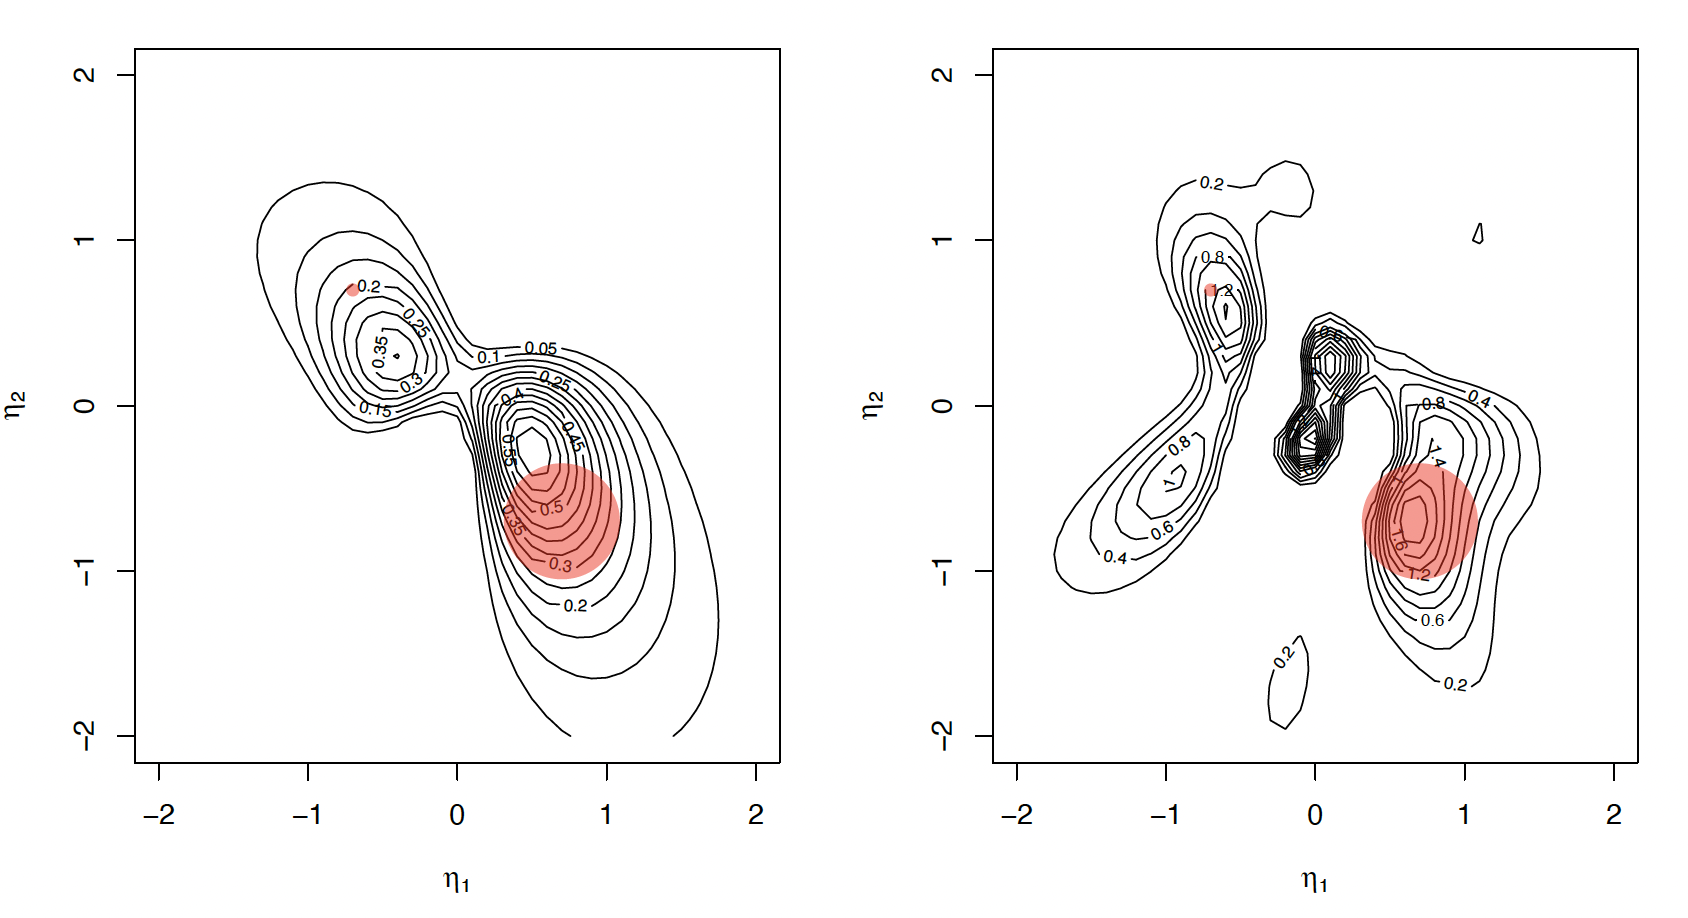
\includegraphics[scale = 0.5]{GK0_new.png}
\caption{Contour plots of Gautier and Kitamura estimated density for the discrete simulation setting with $\eta$ generated with unequal probabilities 0.1 and 0.9 from the two points  (0.7,-0.7) and (-0.7,0.7) indicated by the red circles. In the left panel the sieve dimension is set at the default value T=3, while in the right panel it is increased to T=7.}
\end{figure}


\begin{figure}[H]
\centering
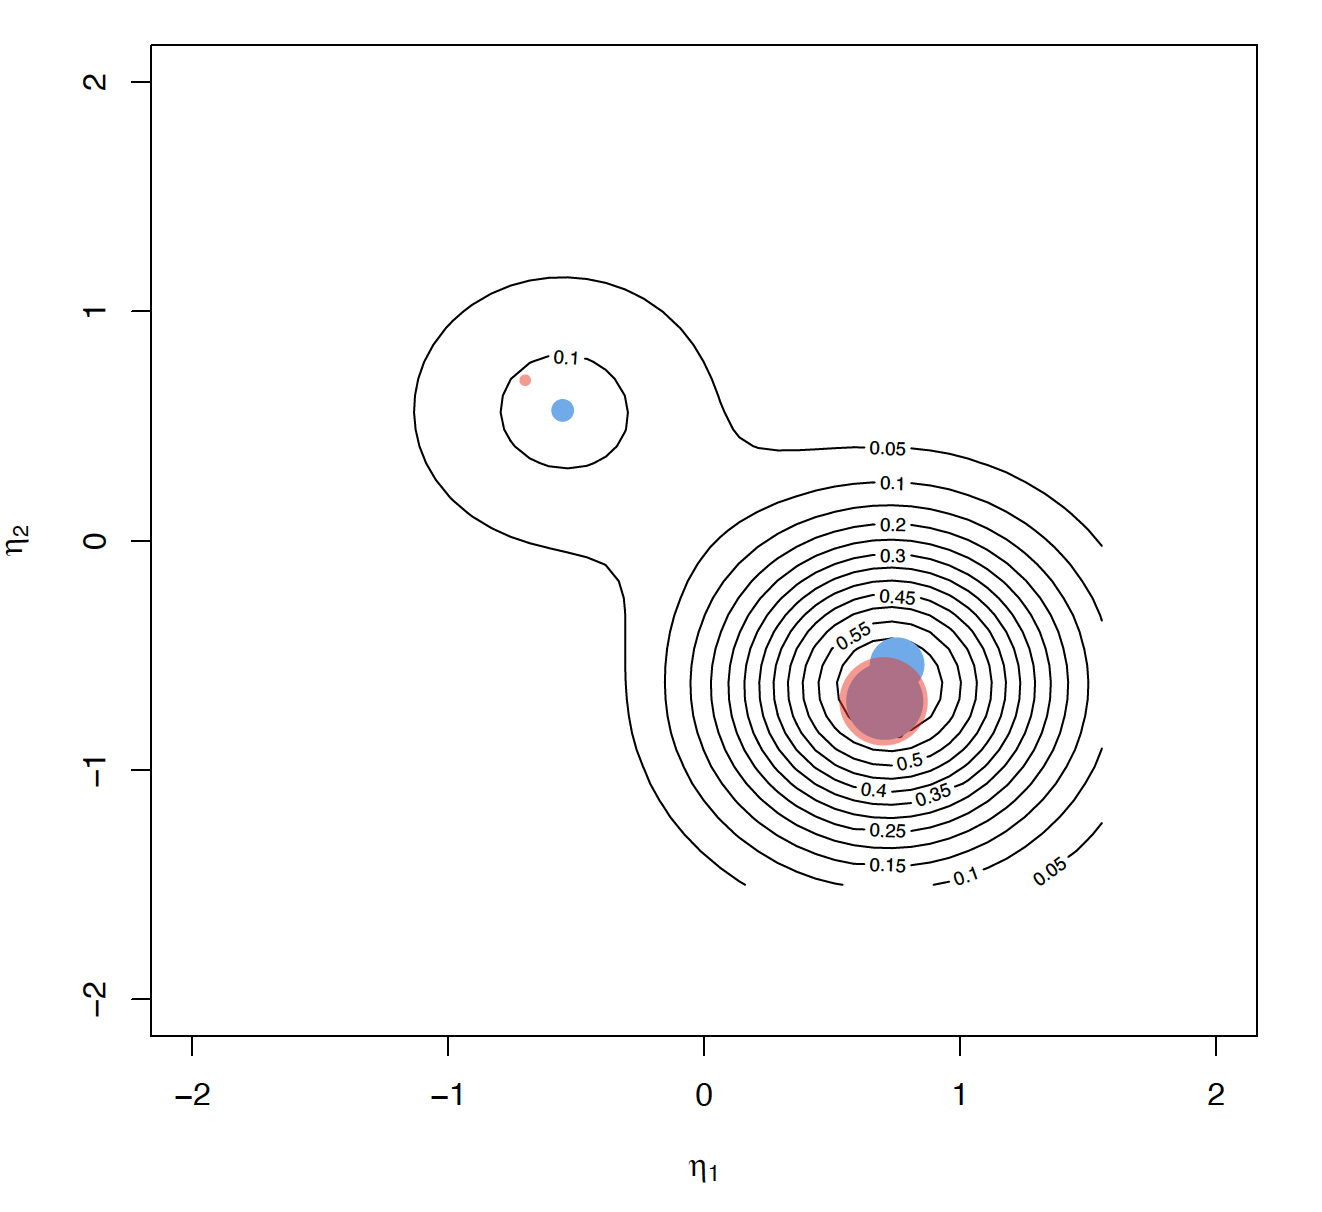
\includegraphics[scale = 0.5]{KW0_new.png}
\caption{Mass points and smoothed contours of the NPMLE for the discrete Gautier–Kitamura simulation setting with unequal masses of 0.1 and 0.9 concentrated at (0.7,-0.7) and (-0.7,0.7) as indicated by the red circles. The mass points of the NPMLE are indicated by the solid blue circles, and contours of a smoothed version of the NPMLE using a bivariate Gaussian kernel.}
\end{figure}



We see in the case of the NPMLE there is very little bias with respect to the larger point mass, with a slight bias when it comes to estimating the location of the smaller point mass. In the case of Gautier and Kitamura's method, the estimated locations of both point masses are biased when the sieve dimension is the default value. This bias seems to decrease as the sieve dimension increases, but this comes with a clear increase in variance.  

\subsection{Bivariate Gaussians}

\indent

Now, we perform a similar adjustment to the second simulation setting in the paper, where the true underlying distribution is a Gaussian mixture of two components at the same points as used above. Again, we will adjust this setting to no longer consider an equal mixture but instead a mixture of weights 0.1 and 0.9. The results can be found below. 

\begin{table}[!htbp]
\begin{center}
\begin{tabular}{lrrrr}
\hline\hline
\multicolumn{1}{l}{}&\multicolumn{1}{c}{GK}&\multicolumn{1}{c}{NPMLE}&\multicolumn{1}{c}{NPMLEs}&\multicolumn{1}{c}{Logit}\tabularnewline
\hline
MAE&$0.24$&$  0.19$&$  0.18$&$0.07$\tabularnewline
RMSE&$0.30$&$  0.25$&$  0.23$&$0.08$\tabularnewline
Time&$8.88$&$206.67$&$206.67$&$0.03$\tabularnewline
\hline
\end{tabular}
\caption{Bivariate Gaussian Simulation Setting:  
Mean Absolute and Root Mean Squared Errors of Predicted Probabilities. 
The computational fitting times reported for NPMLE and NPMLEs are the same as the smoothing occurs only during the prediction process.}
\label{tab.sim1a}
\end{center}
\end{table}


Similar to the prior example, we see that the the method proposed by Gautier and Kitamura seems to be outperformed by the NPMLE method at the sample size of $n = 100$. This case, however, does result in the NPMLE method getting outperformed by logistic regression. The large discrepancy in computational times is again seen here. As before, contour plots of the corresponding density estimates for the GK and NPMLE methods can be found in Figure 3 and Figure 4 respectively. 

\begin{figure}[H]
\centering
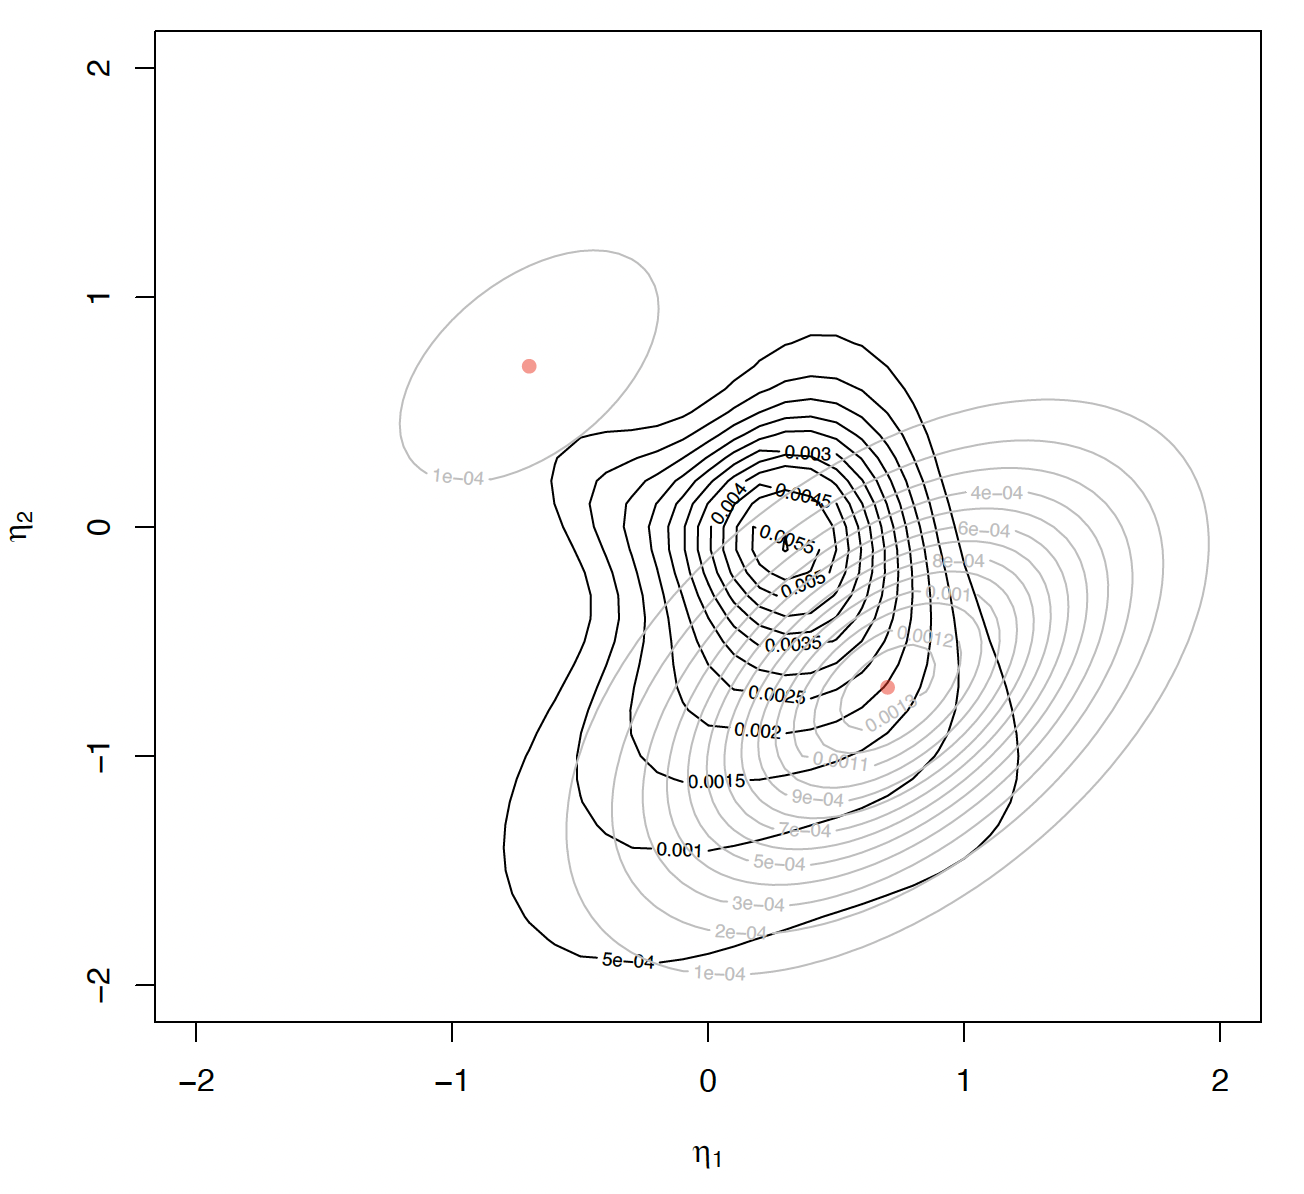
\includegraphics[scale = 0.5]{GK1_new.png}
\caption{Contour plots of Gautier and Kitamura estimated density for the bivariate gaussian simulation setting with $\eta$ generated with unequal probabilities 0.1 and 0.9 centered at the two points  (0.7,-0.7) and (-0.7,0.7) indicated by the red circles. The sieve dimension is set at the default value T=3.}
\end{figure}


\begin{figure}[H]
\centering
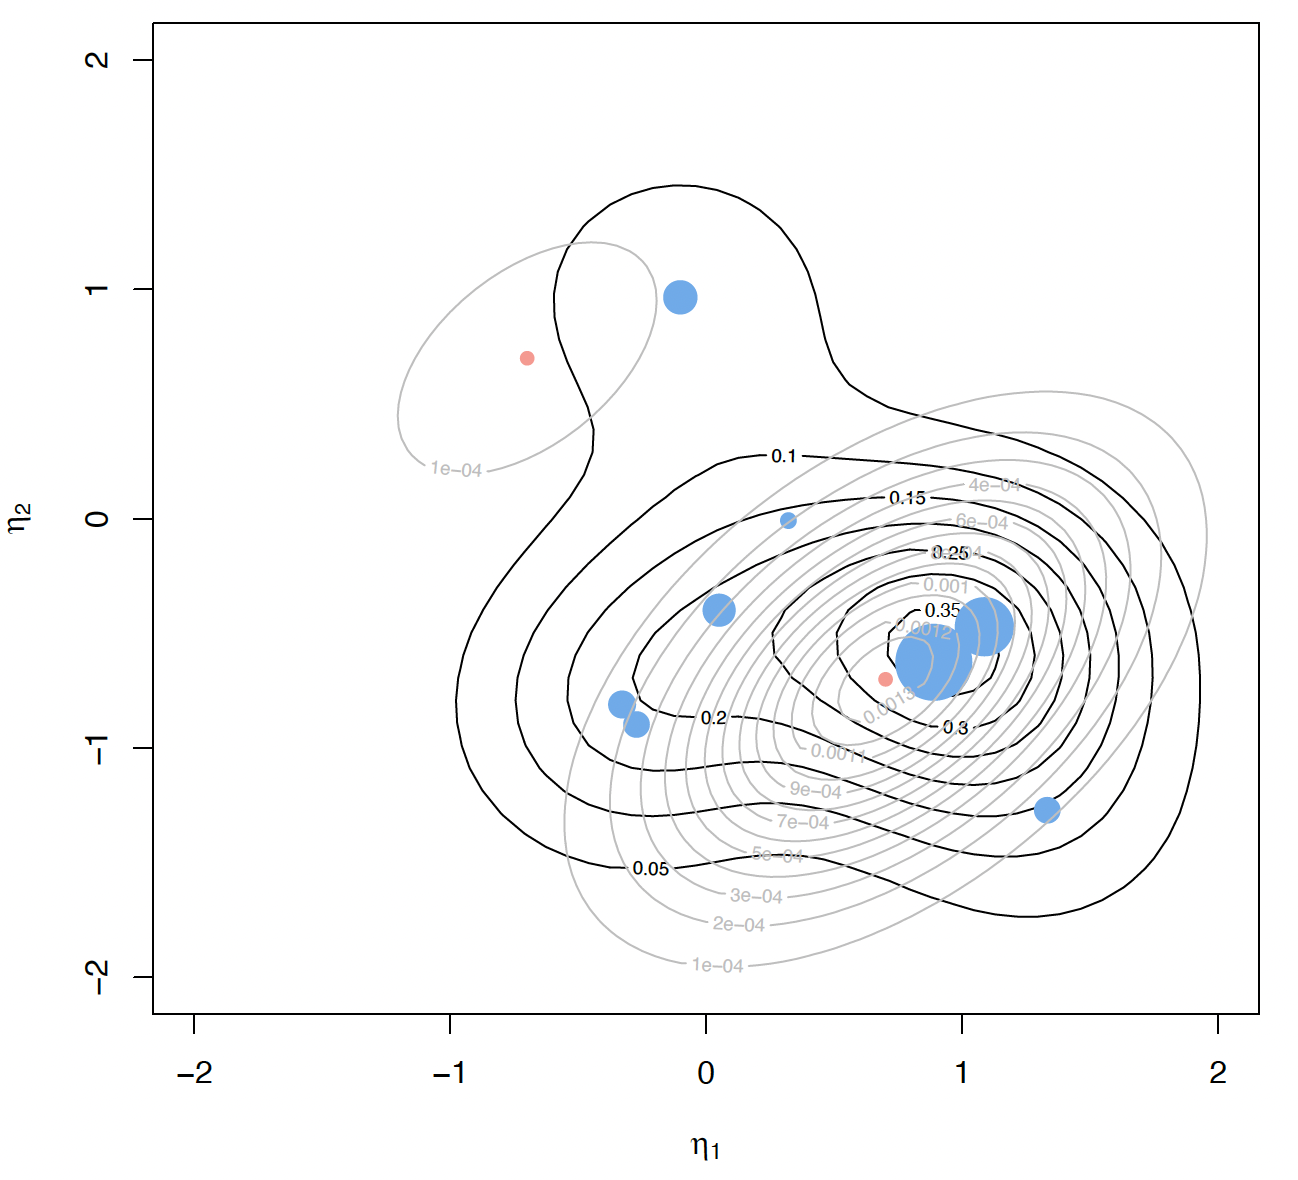
\includegraphics[scale = 0.5]{KW1_new.png}
\caption{Mass points and smoothed contours of the NPMLE for the bivariate gaussian Gautier–Kitamura simulation setting with unequal masses of 0.1 and 0.9 centered at (0.7,-0.7) and (-0.7,0.7) as indicated by the red circles. The mass points of the NPMLE are indicated by the solid blue circles, and contours of a smoothed version of the NPMLE using a bivariate Gaussian kernel.}
\end{figure}

We still see some bias in the NPMLE estimates of the true peaks of the underlying distribution, especially with respect to the smaller peak. This bias is even more present in the countour plot of the Gautier and Kitamura estimate, as only one peak was reported in that case. Note that this bias would likely decrease with an increase in the sieve dimension.

\section{Discussion}

The NPMLE framework developed in \cite{NPMLE} provides non-parametric strongly consistent estimators for underlying distributions within binary response models. We have explored these proofs of strong consistency in further detail, highlighting the usage of concepts relevant to our coursework.  

The clearest limitation of this framework is the current computational inefficiency of its optimization. Additionally, while the NPMLE is able to outperform the Gautier and Kitamura estimator in both cases presented, it is outperformed by logistic regression in the case of an extreme underlying bivariate gaussian mixture. A further study could incorporate cross-validation for determining the optimal tuning parameters of the Gautier and Kitamura estimator instead of simply using the suggested values. It would be interesting to see if that brings the overall computational time of the Gautier and Kitamura estimator close to that of the NPMLE, or if the algorithm for the NPMLE would still remain much more computationally intensive. Additionally, further examination of these settings at larger Monte Carlo simulations and sample sizes would be ideal. 

\begin{singlespace}
	\bibliographystyle{rss}
	\bibliography{refs}
\end{singlespace}

\end{document}



